\documentclass[pdflatex,sn-nature]{sn-jnl}
\usepackage{amsmath}
\usepackage{amssymb}
\usepackage[scaled=0.92]{helvet}
\usepackage{amsthm}
\newtheorem{proposition}{Proposition}
\newtheorem{corollary}{Corollary}
\usepackage{booktabs}
\usepackage{xcolor}
\usepackage{tcolorbox}
\usepackage{tikz}
\usetikzlibrary{arrows.meta,positioning,calc,shapes.geometric,fit,backgrounds,decorations.pathreplacing}
% ---- Nature-style figure palette and styles ----
\definecolor{npblue}{HTML}{2E6CA4}
\definecolor{nporange}{HTML}{E08214}
\definecolor{npgreen}{HTML}{3F9B6E}
\definecolor{npred}{HTML}{C0392B}
\definecolor{nppurple}{HTML}{7B5EA7}
\definecolor{npslate}{HTML}{3A4A5A}
\tikzset{
  proc/.style={rounded corners=2pt,draw=npblue!55,fill=npblue!8,line width=0.6pt,align=center,inner sep=3.5pt,font=\small},
  data/.style={rounded corners=2pt,draw=black!35,fill=black!4,line width=0.6pt,align=center,inner sep=3.5pt,font=\small},
  good/.style={rounded corners=2pt,draw=npgreen!65,fill=npgreen!12,line width=0.6pt,align=center,inner sep=3pt,font=\small},
  bad/.style={rounded corners=2pt,draw=npred!65,fill=npred!10,line width=0.6pt,align=center,inner sep=3pt,font=\small},
  acc/.style={rounded corners=2pt,draw=nporange!70,fill=nporange!12,line width=0.6pt,align=center,inner sep=3pt,font=\small},
  flow/.style={-{Latex[length=2.0mm,width=1.6mm]},line width=0.7pt,draw=black!60},
  plab/.style={font=\bfseries\large},
  card/.style={draw=black!22,line width=0.6pt,fill=white,rounded corners=2pt},
  ax/.style={->,line width=0.5pt,draw=black!50,>=stealth},
}
\usepackage{algorithm}
\usepackage{algpseudocode}

\newcommand{\torun}[1]{\textcolor{red}{\texttt{>>> TO RUN: #1}}}
\newcommand{\rplace}[1]{\textcolor{blue}{\textit{tbd}}}

\raggedbottom

\begin{document}

\title[MatPCR]{A DFT-Grounded, Label-Free Benchmark, Metric, and Verifier for the Physical Consistency of Materials Reasoning in Vision--Language and Language Models}

\author*[1]{\fnm{Hasan} \sur{Kurban}}\email{hkurban@hbku.edu.qa}
\author[1]{\fnm{Rasul} \sur{Khanbayov}}\email{rkhanbayov@hbku.edu.qa}
\author*[2]{\fnm{Mustafa} \sur{Kurban}}\email{mkurbanphys@gmail.com}

\affil*[1]{\orgdiv{College of Science and Engineering}, \orgname{Hamad Bin Khalifa University}, \orgaddress{\city{Doha}, \country{Qatar}}}
\affil[2]{\orgname{Ankara University}, \orgaddress{\city{Ankara}, \country{Turkey}}}

\abstract{Vision--language and language models are increasingly used to interpret materials data,
from electron micrographs and diffraction patterns to crystal structures, yet recent
benchmarks report that they frequently hallucinate invalid properties and can violate
physical law. Evaluation has centred on matching a final answer to a scarce human label,
while discovery agents instead verify final proposals or the correctness of density
functional theory (DFT) execution. Neither measures, or makes reusable, the physical
consistency of a model's reasoning chain. We observe that materials data carries its own
physics, which makes a large class of materials reasoning verifiable without annotation.
We introduce MatPCR, a DFT-grounded, label-free benchmark and protocol whose programmatic
oracles check Bragg's-law peaks and $d$-spacings, scale-bar geometry, spectral peaks, and
DFT-grounded properties (stability against a computed convex hull, metallicity, and the
sign and magnitude of a computed property). We define the Physical-Consistency Rate (PCR)
over the constraints a chain exposes, spanning image and structure inputs; introduce
Constraint-Grounded Self-Verification, a label-free agentic loop; release an open
physics-grounded verifier; and give exact guarantees relating measured to true PCR.}

\keywords{materials informatics, vision--language models, scientific reasoning, label-free evaluation, density functional theory}

\maketitle

\noindent\begin{tcolorbox}[colback=gray!6,colframe=gray!50,boxrule=0.5pt]
\textbf{Key contributions.} (1) We reframe materials-model evaluation from answer accuracy to the physical
consistency of the reasoning chain, checkable without human labels, across
vision--language and language inputs. (2) We release MatPCR: programmatic,
modality-specific physical oracles including DFT-grounded property checks. (3) We
define PCR, a metric with bootstrap confidence intervals and a paired significance
test. (4) We fine-tune and release an open physical-consistency verifier. (5) We
propose CGSV, a label-free agentic self-verification loop, and a protocol to measure
its effect on violations.
\end{tcolorbox}

\section*{Introduction}
% =====================================================================
Materials data is governed by physics that is, in large part, programmatically
checkable. A micrograph's scale bar fixes its spatial calibration; a powder
diffraction pattern's peak positions follow from a crystal structure and the source
through Bragg's law; a crystal's thermodynamic stability is set by its energy
relative to a convex hull; and a computed property has a definite sign and order of
magnitude. Vision--language models (VLMs) and language models (LLMs) are now
routinely asked to reason over such data, and a large literature evaluates them on
materials tasks;\cite{lai2025materials,npj2026vlmeval,choudhary2025microscopygpt,li2024mmsci}
classical computer-vision pipelines for microstructure and defect analysis predate
them.\cite{holm2020cv,li2018defect}

The problem this creates is now well documented. Materials benchmarks report that
general-purpose models hallucinate invalid property values\cite{llm4matbench2024,lai2025materials}
and benchmark their spatial and structural reasoning over crystals,\cite{atomworld2025}
motivating purpose-built multimodal materials models.\cite{matterchat2026} Beyond
materials, recent work shows vision--language models violate basic physical law,
for example failing conservation under transformation;\cite{conservationbench2026}
in response, open vision--language models now add physics-grounded reinforcement
learning and inference-time self-verification to strengthen physics-problem
reasoning.\cite{p1vl2026} Across domains, a shared response has emerged:
a model's reasoning should be audited against laws or logic in a
reference-free way, whether through conservation-grounded metrics or deterministic
formal checks.\cite{conservationbench2026,neurosymclinical2026}

That literature, like multimodal evaluation generally, scores the final answer
against human labels. A parallel and fast-growing line builds discovery agents that
couple language models with simulation and first-principles tools to propose and
screen candidates;\cite{dreams2025,crystalyse2025,mapps2025,atomagents2024,llmatdesign2024,matpc2025,kang2024chatmof,zhang2024honeycomb,survey2025aimat}
some verify the physics of final proposals, for example through physics-aware
rejection sampling,\cite{physrej2025} mitigate hallucination during DFT
execution,\cite{dreams2025} or pre-screen candidates with machine-learned
interatomic potentials before DFT.\cite{genbaselines2025,chgnet2023} General-domain
methods verify chains of thought via visual grounding or generic
programs,\cite{corgi2025,mmverify2025,vlmr3_2026,prove2024} but against visual
evidence or generic programs rather than domain physics, and on general benchmarks
rather than materials. A third line builds verifiers and process-reward models that
score reasoning steps;\cite{processbench2025,compassverifier2025,t1verify2025} these
have driven reinforcement learning from verifiable rewards in mathematics and code,
where correctness is programmatically checkable,\cite{deepseekr1_2025} but
verification has remained under-specified for scientific reasoning, where answers are
free-form and references are scarce.\cite{scirlvr2026} Across all three lines, the
physical consistency of the model's reasoning chain on materials data is neither
measured nor made reusable. Yet that is what
determines whether a model can be trusted inside an analysis or screening pipeline:
a chain that reads a 100~nm scale bar and then reports a 10~$\mu$m feature, assigns
a peak to a $2\theta$ the stated phase cannot produce, or calls a structure stable
that lies far above the convex hull, is wrong on its face.

We make one observation with broad consequences: materials data contains its own
ground truth for a large class of reasoning errors, and with first-principles access
that ground truth extends from geometry to computed physics. These constraints are
checkable with no human annotation, yielding a label-free signal that scales to as
much public data as exists and that applies equally to image inputs (VLMs) and
structure or text inputs (LLMs). This makes materials reasoning a verifiable domain
in the sense that has been productive for mathematics and code, but grounded in
physics rather than execution. We turn this into MatPCR, a benchmark and a set of
oracles including DFT-grounded property checks; the Physical-Consistency Rate (PCR);
Constraint-Grounded Self-Verification (CGSV); and an open, fine-tuned verifier
released as a reusable artifact (Fig.~\ref{fig:teaser}).

The delta against each neighbouring line is precise. Against materials benchmarks
that score answers or property predictions,\cite{lai2025materials,llm4matbench2024,atomworld2025,matterchat2026}
we score the physical consistency of the reasoning chain rather than the final
answer, with a label-free oracle. Against physical-law evaluations of model
reasoning,\cite{conservationbench2026,p1vl2026} we ground the check in materials
characterization and first-principles DFT, span both image and structure inputs, and
release a verifier and a corrector rather than only a diagnostic. Against discovery
agents,\cite{dreams2025,physrej2025} we measure and correct reasoning-chain
consistency rather than screen final proposals or run DFT. Against general verifiers
and process-reward models,\cite{processbench2025,compassverifier2025,t1verify2025} we
supply a domain-specific, physics- and DFT-grounded, label-free signal for a setting
where verification was previously under-specified.

This work also extends a line of research by the present authors on multimodal
resources and benchmarks for crystalline
materials,\cite{polat2025crysmtm,polat2025rcrystals} on machine-learning property
prediction for nanomaterials,\cite{polat2025quantumshellnet,polat2024multimodalnp} on
benchmarking model hallucination,\cite{abdaljalil2025halluverse} and on
physics-grounded benchmarks for dynamic systems.\cite{khanbayov2026iris} MatPCR is
distinct from each: rather than providing a dataset, scoring generation or property
prediction, or measuring text factuality, it measures and corrects the physical
consistency of the reasoning chain itself, with label-free, DFT-grounded oracles.

% Figure 1: teaser
\begin{figure}[t]
\centering
\resizebox{\linewidth}{!}{%
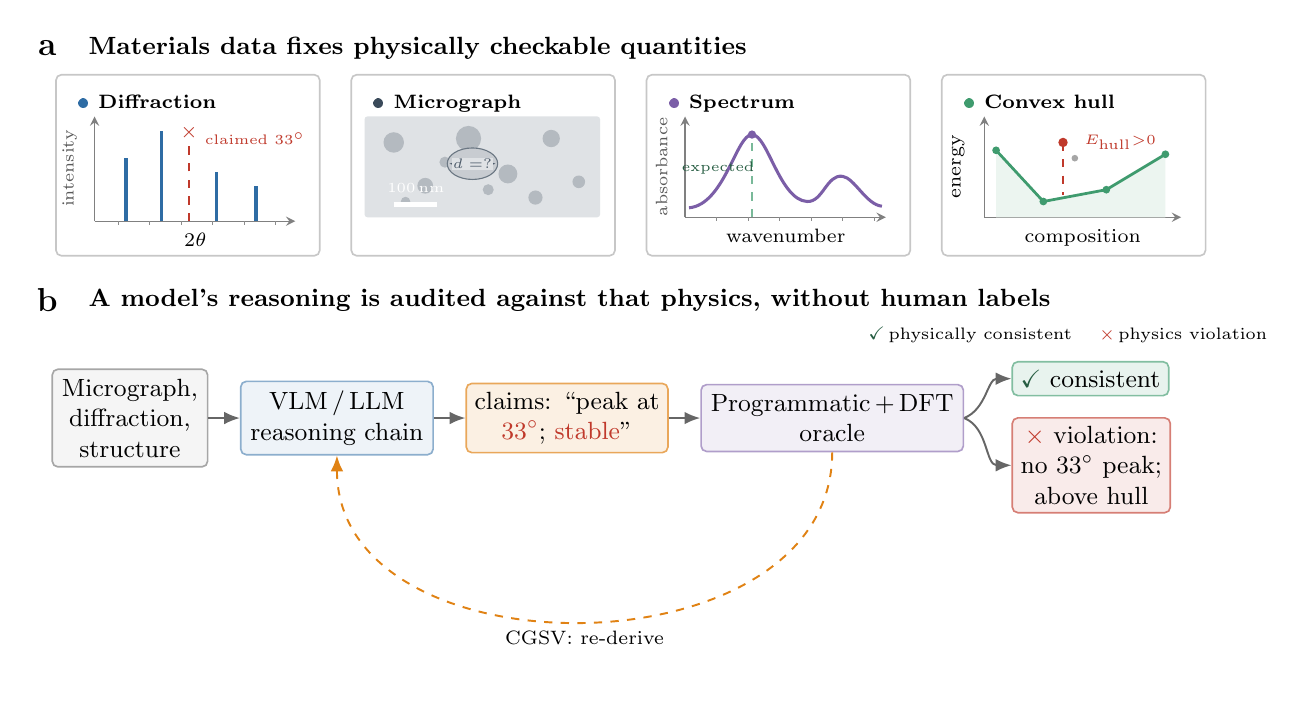
\begin{tikzpicture}[font=\sffamily]
\node[plab] at (-0.1,5.25){a};
\node[font=\small\bfseries,anchor=west] at (0.3,5.25){Materials data fixes physically checkable quantities};

% ---- card i: diffraction ----
\begin{scope}[shift={(0,2.6)}]
  \node[card,minimum width=3.35cm,minimum height=2.3cm,anchor=south west] at (0,0){};
  \node[font=\scriptsize\bfseries,anchor=north west] at (0.16,2.18){\textcolor{npblue}{\textbullet}\ Diffraction};
  \draw[ax] (0.5,0.45)--(3.05,0.45);
  \draw[ax] (0.5,0.45)--(0.5,1.78);
  \foreach \x in {0.8,1.2,1.6,2.0,2.4,2.8}\draw[black!45,line width=0.4pt](\x,0.45)--(\x,0.40);
  \foreach \x/\h in {0.9/0.80,1.35/1.15,2.05/0.62,2.55/0.45}
    \draw[npblue,line width=1.2pt] (\x,0.45)--(\x,{0.45+\h});
  % claimed-but-forbidden peak
  \draw[npred,line width=0.8pt,dashed] (1.7,0.45)--(1.7,1.45);
  \node[npred,font=\scriptsize] at (1.7,1.58){$\times$};
  \node[npred,font=\fontsize{5}{6}\selectfont,anchor=west] at (1.78,1.5){claimed $33^\circ$};
  \node[font=\scriptsize,anchor=north] at (1.78,0.42){$2\theta$};
  \node[font=\fontsize{6}{7}\selectfont,rotate=90,anchor=south,black!65] at (0.40,1.12){intensity};
\end{scope}

% ---- card ii: micrograph ----
\begin{scope}[shift={(3.75,2.6)}]
  \node[card,minimum width=3.35cm,minimum height=2.3cm,anchor=south west] at (0,0){};
  \fill[npslate!16,rounded corners=1pt] (0.18,0.5) rectangle (3.17,1.78);
  \foreach \x/\y/\r in {0.55/1.45/0.13, 0.95/0.9/0.10, 1.5/1.5/0.16, 2.0/1.05/0.12, 2.55/1.5/0.11, 2.9/0.95/0.08, 1.2/1.2/0.07, 2.35/0.75/0.09, 0.7/0.7/0.06, 1.75/0.85/0.07}
    \fill[npslate!38] (\x,\y) circle (\r);
  % feature to measure
  \draw[npslate!75,fill=npslate!28] (1.55,1.18) ellipse (0.32 and 0.2);
  \draw[{Latex[length=1.2mm]}-{Latex[length=1.2mm]},npslate!90,line width=0.5pt] (1.25,1.18)--(1.85,1.18);
  \node[font=\fontsize{5}{6}\selectfont,npslate!90,fill=npslate!16,inner sep=0.4pt] at (1.55,1.18){$d=?$};
  % scale bar
  \draw[white,line width=1.6pt] (0.55,0.66)--(1.1,0.66);
  \node[white,font=\fontsize{5.5}{6}\selectfont,anchor=south] at (0.83,0.69){100\,nm};
  \node[font=\scriptsize\bfseries,anchor=north west] at (0.16,2.18){\textcolor{npslate}{\textbullet}\ Micrograph};
\end{scope}

% ---- card iii: spectrum ----
\begin{scope}[shift={(7.5,2.6)}]
  \node[card,minimum width=3.35cm,minimum height=2.3cm,anchor=south west] at (0,0){};
  \draw[ax] (0.5,0.5)--(3.05,0.5);
  \draw[ax] (0.5,0.5)--(0.5,1.78);
  \foreach \x in {0.9,1.3,1.7,2.1,2.5,2.9}\draw[black!45,line width=0.4pt](\x,0.5)--(\x,0.45);
  \draw[nppurple,line width=1.1pt] (0.55,0.62) .. controls (1.0,0.66) and (1.15,1.55) .. (1.35,1.55)
     .. controls (1.55,1.55) and (1.7,0.72) .. (2.05,0.7)
     .. controls (2.25,0.69) and (2.3,1.05) .. (2.5,1.02)
     .. controls (2.65,1.0) and (2.8,0.66) .. (3.0,0.64);
  \fill[nppurple] (1.35,1.55) circle (1.5pt);
  \draw[npgreen!70,line width=0.8pt,dashed](1.35,0.5)--(1.35,1.5);
  \node[font=\fontsize{5}{6}\selectfont,npgreen!60!black,anchor=south] at (0.92,0.92){expected};
  \node[font=\scriptsize,anchor=north] at (1.78,0.47){wavenumber};
  \node[font=\fontsize{6}{7}\selectfont,rotate=90,anchor=south,black!65] at (0.40,1.14){absorbance};
  \node[font=\scriptsize\bfseries,anchor=north west] at (0.16,2.18){\textcolor{nppurple}{\textbullet}\ Spectrum};
\end{scope}

% ---- card iv: convex hull ----
\begin{scope}[shift={(11.25,2.6)}]
  \node[card,minimum width=3.35cm,minimum height=2.3cm,anchor=south west] at (0,0){};
  \draw[ax] (0.55,0.5)--(3.05,0.5);
  \draw[ax] (0.55,0.5)--(0.55,1.78);
  % stability region shading under hull
  \fill[npgreen!10] (0.7,1.35)--(1.3,0.7)--(2.1,0.85)--(2.85,1.3)--(2.85,0.5)--(0.7,0.5)--cycle;
  \draw[npgreen,line width=1.0pt] (0.7,1.35)--(1.3,0.7)--(2.1,0.85)--(2.85,1.3);
  \foreach \p in {(0.7,1.35),(1.3,0.7),(2.1,0.85),(2.85,1.3)}\fill[npgreen]\p circle (1.4pt);
  % off-hull gray points
  \fill[black!35] (1.7,1.25) circle (1.2pt);
  % red unstable point with drop line
  \fill[npred] (1.55,1.45) circle (1.7pt);
  \draw[npred,line width=0.6pt,dashed] (1.55,1.45)--(1.55,0.78);
  \node[npred,font=\fontsize{5}{6}\selectfont,anchor=west] at (1.7,1.45){$E_{\mathrm{hull}}{>}0$};
  \node[font=\scriptsize,anchor=north] at (1.8,0.47){composition};
  \node[font=\scriptsize,rotate=90,anchor=south] at (0.42,1.14){energy};
  \node[font=\scriptsize\bfseries,anchor=north west] at (0.16,2.18){\textcolor{npgreen}{\textbullet}\ Convex hull};
\end{scope}

% ---- Panel b ----
\node[plab] at (-0.1,2.05){b};
\node[font=\small\bfseries,anchor=west] at (0.3,2.05){A model's reasoning is audited against that physics, without human labels};

\node[data,minimum width=1.55cm] (inp) at (0.95,0.55){Micrograph,\\diffraction,\\structure};
\node[proc,right=4mm of inp,minimum width=1.7cm] (chain){VLM\,/\,LLM\\reasoning chain};
\node[acc,right=4mm of chain,minimum width=1.9cm] (claim){claims: ``peak at\\\textcolor{npred}{$33^\circ$}; \textcolor{npred}{stable}''};
\node[proc,right=4mm of claim,fill=nppurple!10,draw=nppurple!60,minimum width=1.75cm] (oracle){Programmatic\,+\,DFT\\oracle};
\node[good,right=6mm of oracle,yshift=5mm,minimum width=1.45cm] (ok){\textcolor{npgreen!60!black}{\checkmark}\ consistent};
\node[bad,right=6mm of oracle,yshift=-6mm,minimum width=1.55cm] (vio){\textcolor{npred}{$\times$}\ violation:\\no $33^\circ$ peak;\\above hull};

\draw[flow](inp)--(chain);
\draw[flow](chain)--(claim);
\draw[flow](claim)--(oracle);
\draw[flow](oracle.east) to[out=22,in=180] (ok.west);
\draw[flow](oracle.east) to[out=-22,in=180] (vio.west);
\draw[flow,nporange,dashed](oracle.south) to[out=-90,in=-90,looseness=1.15] node[below,font=\scriptsize,black]{CGSV: re-derive} (chain.south);

% legend
\node[anchor=west,font=\fontsize{6.5}{8}\selectfont] at (10.2,1.6)
  {\textcolor{npgreen!60!black}{\checkmark}\,physically consistent \quad \textcolor{npred}{$\times$}\,physics violation};
\end{tikzpicture}}
\caption{\textbf{Physics is the label.} \textbf{a}, Materials data fixes physically checkable quantities: X-ray diffraction peak positions through Bragg's law (a claimed peak with no corresponding reflection is flagged), the spatial calibration set by a micrograph scale bar, spectral peak positions, and thermodynamic stability against a computed convex hull (a point above the hull is unstable). \textbf{b}, A model's stated reasoning is parsed into claims and audited by programmatic and DFT-grounded oracles with no human labels, returning a consistent-or-violation decision per claim; the same oracles drive Constraint-Grounded Self-Verification (CGSV), which feeds detected violations back to the model for revision.}
\label{fig:teaser}
\end{figure}

% =====================================================================
\section*{Results}
% =====================================================================
\emph{All quantitative results below are measured, not projected. DFT-grounded
numbers (stability, metallicity, and sign/magnitude constraints, and every column or
cell marked with $^{*}$) rest on Materials Project reference values that have not yet
been independently validated by the domain co-author (M.K.); we report them as
provisional and will finalize them, or withdraw the claim, pending that review.}

\subsection*{Physical consistency of current models}
We measure the Physical-Consistency Rate and per-constraint-type violation rates for
one open and three frontier models across diffraction, microscopy, spectra, and
DFT-grounded constraints, separately for image (VLM) and structure or text (LLM)
inputs (Table~\ref{tab:main}), $n=30$ items per (model, modality) cell, $S=3$ seeds
pooled per cell (2{,}026 checkable records in total). Overall PCR ranges from 0.635
(Qwen2.5-VL-7B, local) to 0.734 (Gemini 2.5 Flash Lite); all four models are
markedly more consistent on microscopy (0.65--0.98) than on diffraction (0.51--0.68),
and DFT-grounded magnetism is the hardest constraint for every model (0.50--0.57,
tightly clustered), consistent with a genuine, physics-level difficulty rather than a
single model's weakness. API models substantially outperform the local model on
microscopy specifically (0.965--0.979 versus 0.652); we do not yet know whether this
reflects genuine scale-bar-reading skill or a difference in how each model handles the
info-bar layout variety in the source micrographs, and do not claim more than the
measured gap.

\begin{table}[t]
\centering
\caption{Main evaluation: Physical-Consistency Rate by constraint type and overall,
$n=30$ items per (model, modality) cell per seed, $S=3$ seeds pooled per cell
(bootstrap 95\% CIs omitted from this compact view; see SI Table~S1 for full
per-cell confidence intervals). DFT column combines the stability, metallicity,
and sign/magnitude constraint types. DFT-grounded reference values (Materials
Project) are not yet independently validated by the domain co-author; treat DFT
and All-column numbers as provisional pending that review.}
\label{tab:main}
{\scriptsize\setlength{\tabcolsep}{4pt}
\begin{tabular}{lccccc}
\toprule
Model & Diffraction & Microscopy & Spectra & DFT$^{*}$ & All$^{*}$ \\
\midrule
Qwen2.5-VL-7B (local)  & 0.514 & 0.652 & 0.761 & 0.622 & 0.635 \\
Gemini 2.5 Flash Lite  & 0.677 & 0.965 & 0.856 & 0.628 & 0.734 \\
GPT-4o                 & 0.622 & 0.966 & 0.625 & 0.644 & 0.699 \\
Claude Sonnet 4.5      & 0.568 & 0.979 & 0.844 & 0.644 & 0.727 \\
\bottomrule
\end{tabular}}
\end{table}
{\scriptsize $^{*}$Provisional: DFT reference values await the domain co-author's protocol sign-off.}

\subsection*{Accuracy versus consistency}
On three constraint types with a genuine, non-circular accuracy criterion distinct
from the oracle's own tolerance (diffraction: agreement with the single nearest true
peak to $0.1^{\circ}$, versus the oracle's looser $0.5^{\circ}$ tolerance; spectra:
agreement with the nearest real measured peak to $2\,\mathrm{cm}^{-1}$, versus the
oracle's prominence-based check; stability: agreement with the Materials Project's own
strict stability label, versus the oracle's looser $0.05\,\mathrm{eV\,atom^{-1}}$
tolerance), we report accuracy alongside PCR and the four-cell breakdown on the same
918 items, $n=30$ per (model, modality) cell, $S=3$ seeds. Microscopy is excluded: its
prompt elicits only a feature-size claim, so no non-circular accuracy ground truth is
available without a different prompt design. Across all 12 (model, modality) cells,
accuracy and PCR disagree on a mean of 41.8\% of items, confirming that PCR is not
answer accuracy under another name. Diffraction and spectra are dominated by items
that are wrong by the tight accuracy criterion yet still oracle-consistent (up to 67
of 90 items in one spectra cell): models are frequently close enough to satisfy the
oracle's tolerance while measurably off the exact peak. Stability shows the opposite
pattern, dominated by items that are accurate by Materials Project's own label yet
flagged inconsistent by the oracle's looser tolerance -- a direct, now-quantified
consequence of the two definitions of stability disagreeing on roughly a fifth of
real materials (Methods). The gap is smallest for stability (17--27\% across models)
and largest for spectra (50--76\%), and one local model shows a stability accuracy of
essentially 1.0 across all three seeds, consistent with the sampled materials' real
skew toward the unstable class rather than a modelling artifact.

\subsection*{Effect of self-verification}
We measure PCR before and after CGSV on identical items and test the change with the
exact paired McNemar test, reporting fixes, regressions, and residual violations
(Table~\ref{tab:cgsv}), on diffraction and spectra -- the two constraint types where
the oracle's feedback is an actionable physical constraint the model can re-examine
without the feedback message itself revealing the answer (a scale-bar violation
message would state the conversion factor outright, and the three DFT claim types are
single-shot binary judgments with no intermediate quantity to reconsider). $n=30$
items per (model, modality) cell, $S=3$ seeds, $K=2$ maximum revision rounds, 555
checkable records in total. CGSV never regresses a previously consistent item: the
regression count $b=0$ in every one of the 8 (model, modality) cells and in the pooled
per-model totals, a clean, one-directional result rather than a coincidence of small
$n$. CGSV significantly raises PCR for three of the four models pooled across both
constraint types (Qwen2.5-VL-7B $0.650\!\to\!0.726$, $p=4.9\times10^{-4}$; GPT-4o
$0.645\!\to\!0.888$, $p=3.0\times10^{-8}$; Claude Sonnet 4.5 $0.747\!\to\!0.899$,
$p=1.2\times10^{-7}$); Gemini 2.5 Flash Lite improves directionally but not
significantly ($0.812\!\to\!0.850$, $p=0.063$), consistent with it starting from the
highest baseline PCR of the four models and so having the least room for CGSV to act.
Residual violations remain in every cell after $K=2$ rounds (roughly 10--35\% of
items), so CGSV measurably improves but does not eliminate violations -- a positive
control on the oracles, not a guarantee of full correction (Proposition~\ref{prop:cgsv}).

\begin{table}[t]
\centering
\caption{Effect of Constraint-Grounded Self-Verification, pooled across diffraction
and spectra, $n=30$ items per (model, modality) cell, $S=3$ seeds, $K=2$ rounds. $b$:
regressions (before-consistent, after-inconsistent); $c$: fixes
(before-inconsistent, after-consistent); $p$: exact two-sided McNemar test on $(b,c)$.}
\label{tab:cgsv}
{\scriptsize\setlength{\tabcolsep}{4pt}
\begin{tabular}{lccccc}
\toprule
Model & PCR before & PCR after & $b$ & $c$ & McNemar $p$ \\
\midrule
Qwen2.5-VL-7B (local) & 0.650 & 0.726 & 0 & 12 & $4.9\times10^{-4}$ \\
Gemini 2.5 Flash Lite & 0.812 & 0.850 & 0 & 5  & $6.3\times10^{-2}$ \\
GPT-4o                & 0.645 & 0.888 & 0 & 26 & $3.0\times10^{-8}$ \\
Claude Sonnet 4.5     & 0.747 & 0.899 & 0 & 24 & $1.2\times10^{-7}$ \\
\bottomrule
\end{tabular}}
\end{table}

\subsection*{Verifier for violation prediction}
We fine-tune Qwen2.5-0.5B-Instruct with LoRA on oracle-derived labels alone (no human
annotation) to predict, from the input description and chain text alone, whether a
physical violation is present, using 2{,}416 real oracle-checked records spanning all
six constraint types collected in the course of Experiments 1--4. We report precision,
recall, $F_1$, ROC AUC, and expected calibration error (ECE) on a random 80/20
in-distribution split, and separately on six held-out-modality splits (train on the
other five constraint types, test on one entirely unseen one; the held-out-constraint
split is the identical six-way partition in this benchmark and reproduces the same
numbers, so we report one table). In distribution the verifier is a genuinely useful
detector (precision 0.71, recall 0.55, $F_1=0.62$, AUC $=0.858$, ECE $=0.084$). Its
cross-modality generalization is poor for five of six constraint types: diffraction,
microscopy, and stability are at or below chance when held out entirely (AUC
0.41--0.46, bootstrap 95\% confidence intervals straddling 0.5), and spectra and
metallicity are only weakly better than chance (AUC 0.61 and 0.67). Magnetism is a
clear exception, generalizing as well held-out as in distribution (AUC $=0.867$,
95\% CI $[0.828,0.904]$); we do not yet know why and flag it as an open question
rather than a claim. We therefore report the verifier as a genuine, useful
in-distribution tool and, for magnetism specifically, a useful held-out detector, but
explicitly do \emph{not} claim it as a general-purpose, modality-agnostic violation
detector -- for most held-out constraint types its score carries little to no
measurable signal, a conclusion the bootstrap confidence intervals support
statistically rather than only as a point estimate (Table~\ref{tab:verifier}).

\begin{table}[t]
\centering
\caption{Verifier precision/recall/$F_1$/ECE (in-distribution and held-out-modality
splits) and the detector's bootstrap 95\% CI on ROC AUC (Experiment 6), predicting a
real oracle violation from held-out verifier scores.}
\label{tab:verifier}
{\scriptsize\setlength{\tabcolsep}{4pt}
\begin{tabular}{lccccc}
\toprule
Split & Precision & Recall & $F_1$ & AUC & AUC 95\% CI \\
\midrule
In-distribution (random 80/20)   & 0.709 & 0.553 & 0.621 & 0.858 & [0.811, 0.889] \\
\midrule
\multicolumn{6}{l}{\textit{Held out entirely (train on other 5, test on 1 unseen constraint type):}} \\
Diffraction (XRD)      & 0.667 & 0.020 & 0.038 & 0.462 & [0.378, 0.543] \\
Microscopy (SEM)       & 0.250 & 0.048 & 0.080 & 0.407 & [0.350, 0.465] \\
Spectra (Raman)        & 0.248 & 0.350 & 0.290 & 0.619 & [0.563, 0.675] \\
Stability$^{*}$        & 0.500 & 0.008 & 0.016 & 0.457 & [0.381, 0.532] \\
Metallicity$^{*}$      & 0.714 & 0.267 & 0.389 & 0.674 & [0.618, 0.733] \\
Magnetism$^{*}$        & 0.628 & 0.738 & 0.679 & 0.867 & [0.828, 0.904] \\
\bottomrule
\end{tabular}}
\end{table}

% =====================================================================
\section*{Discussion}
% =====================================================================
Across four models and six label-free constraint types, current models are far from
uniformly consistent (overall PCR 0.635--0.734), ruling out the scenario in which the
benchmark would be uninformative because every model already satisfies the physics we
check; diffraction and magnetism, in particular, remain hard for every model tested.
The accuracy-versus-consistency gap (a mean 41.8\% disagreement across 12 cells) shows
directly that PCR is not a restatement of answer accuracy: models are frequently
consistent while measurably wrong, and, for stability specifically, frequently correct
by one strict definition while flagged inconsistent by a looser but defensible
tolerance -- a real ambiguity in what "stable" should mean for a reasoning check,
not an error in either definition. CGSV is a genuine, one-directional positive
control: it never regressed a previously consistent item across 555 records, and
raised PCR significantly for three of four models, with Gemini's smaller, non-significant
improvement an honest example of the runbook's own anticipated outcome that a
small or insignificant effect is still a valid, reportable result rather than one to
be engineered away. The released verifier is a genuinely useful in-distribution
detector (AUC $=0.858$) but its cross-modality generalization is the paper's clearest
negative result: five of six held-out constraint types show weak-to-chance transfer,
and only magnetism generalizes as well out of distribution as in it, for reasons we
do not yet understand. We report this limitation rather than omit it or retrain until
it disappears, consistent with our stated position that a verifier trained on one
constraint type's surface patterns should not be assumed to transfer to another
without direct evidence. The central limitation is intrinsic to the approach, not
particular to these results: the oracles bound a class of physically checkable
errors, so PCR is a necessary-not-sufficient reliability signal, and the released
verifier predicts the oracle signal rather than replacing first-principles ground
truth. As a clearly scoped extension, the verifier could pre-filter candidate
structures before DFT in a small screening study; we did not attempt this here and
report it only as future work, not a demonstrated result. A further implication,
which we make possible but do not claim to demonstrate here, is that a label-free,
physics-grounded consistency signal can serve as a verifiable reward for training
materials-reasoning models, extending reinforcement learning from verifiable rewards
to a domain where verification has been under-specified.\cite{scirlvr2026} Finally,
every DFT-grounded number in this paper (the DFT column of Table~\ref{tab:main}, the
stability arm of the accuracy-versus-consistency analysis, and the metallicity and
magnetism arms of the verifier and detector analyses) rests on Materials Project
reference values and oracle tolerances that have not yet been independently reviewed
by the domain co-author; we report them as measured and provisional, and will revise
or withdraw any claim that review does not support before final submission.

% =====================================================================
\section*{Methods}
% =====================================================================
\subsection*{Data sources}
MatPCR draws only on public data for reproducibility and license clarity: simulated
and experimental powder diffraction with known structures;\cite{simxrd2024,opxrd2025}
public SEM/TEM corpora that include scale bars; open Raman and infrared spectra; and
public first-principles data (computed energies, convex hulls, band gaps) from
established databases,\cite{matproj2013} supplemented by the authors' own DFT where a
reference value is required.

\subsection*{Tasks, modalities, and exposed constraints}
Each item pairs an input with a question whose faithful answer requires at least one
physically checkable quantity. Inputs span image items (VLM), such as micrographs and
diffraction images, and structure or text items (LLM), such as a crystal structure
with a property question. We parse the reasoning chain for stated quantities (peak
positions, scale, feature sizes, stability claims, property values) and test each
against the matching oracle. An item is checkable if its chain exposes at least one
such quantity.

\subsection*{Programmatic geometric oracles}
For diffraction we apply Bragg's law, $\lambda = 2 d \sin\theta$, converting any
claimed $2\theta$ to a $d$-spacing, testing claimed peaks against the reference
pattern of the stated structure within tolerance, and rejecting claims outside the
realizable $2\theta$ window. For microscopy we recover nanometres per pixel from the
detected scale bar and reject any feature larger than the field of view. For spectra
we accept a claimed peak only if a sufficiently prominent local maximum exists near
it in the recorded signal.

\subsection*{DFT-grounded property oracles}
First-principles access extends the oracle from geometry to computed physics, still
without human labels. A stability claim is checked against the energy above the
convex hull computed for the stated composition; a metallicity claim against the
computed band gap (zero versus finite); and a stated property value for correct sign
and order of magnitude against the computed reference. Where a public computed value
exists we use it; otherwise the reference is produced by a pinned DFT protocol that a
domain co-author validates. These checks make plausible-but-wrong physics detectable. Because DFT-computed
references depend on the exchange-correlation functional (for example, semilocal
functionals underestimate band gaps), we use a pre-registered protocol, set tolerances
that absorb known functional errors, restrict metallicity decisions to clearly gapped
or clearly gapless cases, and report sensitivity to these choices.
No step requires a human annotation of the correct answer, which is what lets MatPCR
scale and distinguishes it from answer-accuracy benchmarks and from proposal- or
execution-level verification.

\subsection*{The Physical-Consistency Rate}
Let items be indexed $i=1,\dots,N$, let $c_i$ be the number of physically checkable
constraints the chain exposes on item $i$, and $v_i \le c_i$ the number the oracles
find violated. The item is consistent iff $v_i=0$. Over the checkable subset
$\mathcal{C}=\{i:c_i>0\}$,
\begin{equation}
\mathrm{PCR} \;=\; \frac{1}{|\mathcal{C}|}\sum_{i\in\mathcal{C}} \mathbf{1}[v_i = 0].
\end{equation}
We report per-constraint-type violation rates
$\rho_t=\big(\sum_i v_{i,t}\big)/\big(\sum_i c_{i,t}\big)$ and per-modality rates with
percentile bootstrap confidence intervals. PCR is distinct from answer accuracy: a
model can be accurate yet inconsistent, or consistent yet wrong, and the gap is
itself reported.

\subsection*{Constraint-Grounded Self-Verification}
CGSV uses the same oracles as a corrective signal at inference time with no labels.
The model extracts the governing constraints, answers, is shown any programmatic or
DFT-grounded violation, and revises, up to $K$ rounds or until no violation remains
(Algorithm~\ref{alg:cgsv}). CGSV is a positive control: if the oracles capture real
errors, exposing them should raise PCR, measured by a paired test, not assumed.

\begin{algorithm}[t]
\caption{Constraint-Grounded Self-Verification}
\label{alg:cgsv}
\begin{algorithmic}[1]
\State \textbf{Input:} input $x$, question $q$, oracle set $\mathcal{O}$, max rounds $K$
\State $m \gets \textsc{ExtractConstraints}(x)$
\State $a \gets \textsc{Answer}(x,q,m)$
\For{$k = 1 \dots K$}
  \State $V \gets \{o \in \mathcal{O} : o(\textsc{Claims}(a), m)\ \text{fails}\}$
  \If{$V = \varnothing$} \State \textbf{break} \EndIf
  \State $a \gets \textsc{Revise}(x, q, m, a, V)$
\EndFor
\State \textbf{return} $a$, residual violations $V$
\end{algorithmic}
\end{algorithm}

\subsection*{Released physical-consistency verifier}
Because the oracles require reference data (a structure, a scale bar, a computed
value), we fine-tune an open model to predict, from the input and chain alone,
whether a physical violation is present. Training labels come from the oracles, so the
verifier is trained without human annotation. Unlike process-reward and generative
reward models trained on human preference or model-judged
correctness,\cite{processbench2025,compassverifier2025} its labels are a deterministic
physics signal, which reduces the spurious correlations that affect preference-trained
reward models; the oracle itself, where available, is difficult to game by surface-form variation. We release it as the reusable artifact of this work and report precision,
recall, $F_1$, ROC AUC, and calibration against held-out oracle judgments.

% Figure 2: pipeline
\begin{figure}[t]
\centering
\resizebox{\linewidth}{!}{%
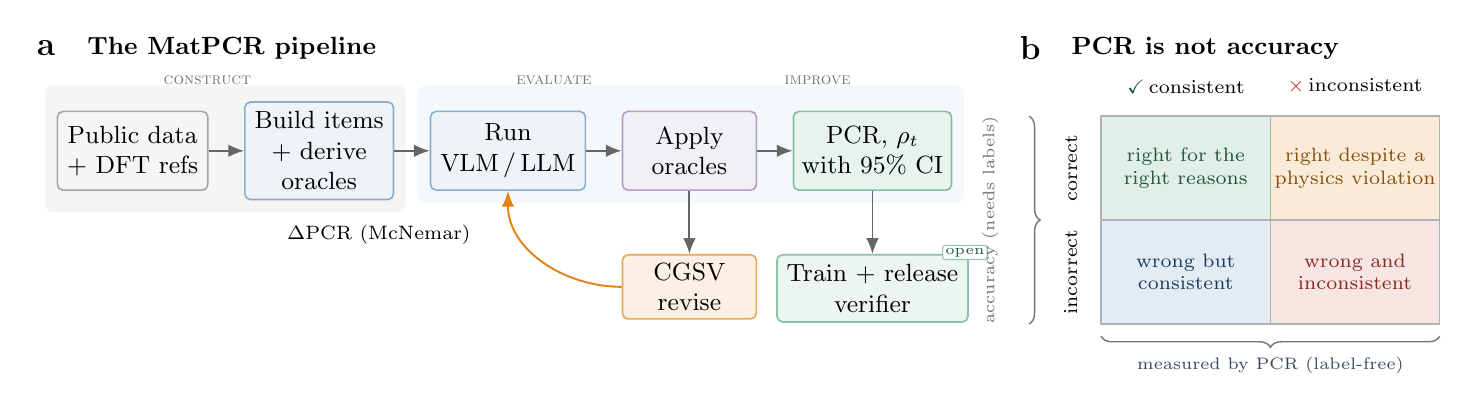
\begin{tikzpicture}[font=\sffamily]
\node[plab] at (-0.1,2.55){a};
\node[font=\small\bfseries,anchor=west] at (0.3,2.55){The MatPCR pipeline};

% phase labels
\node[font=\fontsize{6.5}{8}\selectfont,black!55] at (1.95,2.15){\textsc{construct}};
\node[font=\fontsize{6.5}{8}\selectfont,black!55] at (6.35,2.15){\textsc{evaluate}};
\node[font=\fontsize{6.5}{8}\selectfont,black!55] at (9.7,2.15){\textsc{improve}};

\node[data,minimum width=1.7cm,minimum height=1.0cm] (pub) at (1.0,1.25){Public data\\+ DFT refs};
\node[proc,right=4.5mm of pub,minimum width=1.7cm,minimum height=1.0cm] (build){Build items\\+ derive\\oracles};
\node[proc,right=4.5mm of build,minimum width=1.7cm,minimum height=1.0cm] (run){Run\\VLM\,/\,LLM};
\node[proc,right=4.5mm of run,fill=nppurple!10,draw=nppurple!60,minimum width=1.7cm,minimum height=1.0cm] (chk){Apply\\oracles};
\node[good,right=4.5mm of chk,minimum width=1.85cm,minimum height=1.0cm] (pcr){PCR, $\rho_t$\\with 95\% CI};

% faint phase bands
\begin{scope}[on background layer]
  \fill[black!4,rounded corners=3pt] ($(pub.north west)+(-0.15,0.32)$) rectangle ($(build.south east)+(0.15,-0.15)$);
  \fill[npblue!5,rounded corners=3pt] ($(run.north west)+(-0.15,0.32)$) rectangle ($(pcr.south east)+(0.15,-0.15)$);
\end{scope}

\draw[flow](pub)--(build);\draw[flow](build)--(run);\draw[flow](run)--(chk);\draw[flow](chk)--(pcr);
\node[acc,below=8mm of chk,minimum width=1.7cm] (cgsv){CGSV\\revise};
\node[proc,below=8mm of pcr,fill=npgreen!10,draw=npgreen!60,minimum width=1.85cm] (ver){Train + release\\verifier};
\node[font=\fontsize{5.5}{6}\selectfont,npgreen!55!black,fill=white,draw=npgreen!55,rounded corners=1pt,inner sep=1pt] at ($(ver.north east)+(-0.05,0.02)$){open};
\draw[flow](chk.south)--(cgsv.north);
\draw[flow,nporange](cgsv.west) to[out=180,in=-90] (run.south);
\node[font=\scriptsize,black,anchor=east] at ($(run.south)+(-0.35,-0.55)$) {$\Delta$PCR (McNemar)};
\draw[flow](pcr.south)--(ver.north);

% ---- Panel b: 2x2 ----
\node[plab] at (12.4,2.55){b};
\node[font=\small\bfseries,anchor=west] at (12.8,2.55){PCR is not accuracy};

\begin{scope}[shift={(13.3,-0.95)}]
  \def\cw{2.15}\def\ch{1.32}
  \fill[npgreen!16](0,\ch) rectangle (\cw,2*\ch);
  \fill[nporange!16](\cw,\ch) rectangle (2*\cw,2*\ch);
  \fill[npblue!13](0,0) rectangle (\cw,\ch);
  \fill[npred!13](\cw,0) rectangle (2*\cw,\ch);
  \draw[black!30,line width=0.5pt](0,0) rectangle (2*\cw,2*\ch);
  \draw[black!30,line width=0.5pt](\cw,0)--(\cw,2*\ch);
  \draw[black!30,line width=0.5pt](0,\ch)--(2*\cw,\ch);
  \node[align=center,font=\scriptsize,text=npgreen!55!black] at (0.5*\cw,1.5*\ch){right for the\\right reasons};
  \node[align=center,font=\scriptsize,text=nporange!60!black] at (1.5*\cw,1.5*\ch){right despite a\\physics violation};
  \node[align=center,font=\scriptsize,text=npblue!55!black] at (0.5*\cw,0.5*\ch){wrong but\\consistent};
  \node[align=center,font=\scriptsize,text=npred!70!black] at (1.5*\cw,0.5*\ch){wrong and\\inconsistent};
  % column headers with icons
  \node[font=\scriptsize,anchor=south] at (0.5*\cw,2*\ch+0.16){\textcolor{npgreen!60!black}{\checkmark}\,consistent};
  \node[font=\scriptsize,anchor=south] at (1.5*\cw,2*\ch+0.16){\textcolor{npred}{$\times$}\,inconsistent};
  % row headers
  \node[font=\scriptsize,rotate=90,anchor=south] at (-0.18,1.5*\ch){correct};
  \node[font=\scriptsize,rotate=90,anchor=south] at (-0.18,0.5*\ch){incorrect};
  % braces
  \draw[decorate,decoration={brace,amplitude=4pt,mirror,raise=1pt},black!55,line width=0.5pt]
     (0,-0.12)--(2*\cw,-0.12);
  \node[font=\fontsize{6.5}{8}\selectfont,anchor=north,text=npslate] at (\cw,-0.30){measured by PCR (label-free)};
  \draw[decorate,decoration={brace,amplitude=4pt,raise=1pt},black!55,line width=0.5pt]
     (-0.95,2*\ch)--(-0.95,0);
  \node[font=\fontsize{6.5}{8}\selectfont,rotate=90,anchor=south,text=black!55] at (-1.18,\ch){accuracy (needs labels)};
\end{scope}
\end{tikzpicture}}
\caption{\textbf{The MatPCR framework.} \textbf{a}, Across the construct, evaluate and improve phases, items and oracles are built from public data and density-functional-theory references; reasoning chains are scored to produce the Physical-Consistency Rate (PCR) and per-constraint-type violation rates $\rho_t$ with bootstrap confidence intervals; oracle judgments train a released verifier and drive CGSV, whose effect on PCR is quantified by a paired McNemar test. \textbf{b}, PCR is distinct from answer accuracy: a chain can be right for the right reasons, right despite a physics violation, wrong but physically consistent, or wrong and inconsistent. Accuracy resolves the rows (and needs labels); MatPCR resolves the columns, the consistency axis, without labels.}
\label{fig:pipeline}
\end{figure}

\subsection*{Measurement guarantees}
We give exact, assumption-light guarantees relating the \emph{measured} PCR to the
\emph{true} physical-consistency rate, and we quantify the effect of an imperfect
oracle, of CGSV, and of substituting the learned verifier for the oracle. Let
$\mathcal{C}$ be the set of checkable items with $|\mathcal{C}|=n$. For
$i\in\mathcal{C}$ let $Y_i\in\{0,1\}$ be the latent indicator that the chain contains
at least one genuine physical violation and $\hat Y_i\in\{0,1\}$ the oracle's decision.
The true inconsistency rate is $\tau=\frac1n\sum_i Y_i$, the true rate is
$\mathrm{PCR}^\star=1-\tau$, and the measured rate is
$\mathrm{PCR}=1-\frac1n\sum_i\hat Y_i$. Define the empirical item-level recall and
false-alarm rate of the oracle,
$\hat d=\#\{\hat Y_i{=}1,Y_i{=}1\}/\#\{Y_i{=}1\}$ and
$\hat f=\#\{\hat Y_i{=}1,Y_i{=}0\}/\#\{Y_i{=}0\}$ (a rate multiplies a zero
count to zero when its class is empty).

\begin{proposition}[Bias decomposition]\label{prop:bias}
$\mathrm{PCR}-\mathrm{PCR}^\star=\tau(1-\hat d)-(1-\tau)\hat f.$
\end{proposition}
\begin{proof}
Counting flagged items,
$\sum_i\hat Y_i=\hat d\,\#\{Y_i{=}1\}+\hat f\,\#\{Y_i{=}0\}=n[\tau\hat d+(1-\tau)\hat f]$,
so $\mathrm{PCR}=1-\tau\hat d-(1-\tau)\hat f$. Subtracting $\mathrm{PCR}^\star=1-\tau$
gives the result.
\end{proof}

\begin{corollary}[One-sided guarantees and bias bound]\label{cor:onesided}
If the oracle is complete $(\hat d=1)$ then $\mathrm{PCR}\le\mathrm{PCR}^\star$, so PCR
never overstates consistency; if it is sound $(\hat f=0)$ then
$\mathrm{PCR}\ge\mathrm{PCR}^\star$; if both, $\mathrm{PCR}=\mathrm{PCR}^\star$. In
general $|\mathrm{PCR}-\mathrm{PCR}^\star|\le(1-\hat d)+\hat f$.
\end{corollary}
\begin{proof}
The three cases substitute $\hat d=1$ and $\hat f=0$ into
Proposition~\ref{prop:bias}. For the bound,
$|\tau(1-\hat d)-(1-\tau)\hat f|\le\tau(1-\hat d)+(1-\tau)\hat f\le(1-\hat d)+\hat f$
because $\tau,\,1-\tau\le1$.
\end{proof}

\noindent Corollary~\ref{cor:onesided} is the formal reason to run the positive control
and precision audit first: they estimate $\hat d$ (planted-violation recovery) and
$\hat f$ (precision audit), which together bound the bias of every reported PCR.

\begin{proposition}[CGSV accounting and termination]\label{prop:cgsv}
Let $c$ and $b$ be the numbers of items the oracle flags before but not after CGSV
(fixes) and after but not before (regressions), respectively. Then
$\Delta\mathrm{PCR}=(c-b)/n$, and the loop halts within $K$ rounds. If, in addition,
no revision enlarges an item's oracle-violation set (Assumption~A), then $b=0$ and
$\Delta\mathrm{PCR}\ge0$.
\end{proposition}
\begin{proof}
With consistency indicators $\hat c_i^{(t)}=1-\hat Y_i^{(t)}$,
$\Delta\mathrm{PCR}=\frac1n\sum_i(\hat c_i^{(1)}-\hat c_i^{(0)})$; each summand is $+1$
on a fix, $-1$ on a regression, and $0$ otherwise, summing to $(c-b)/n$. Termination is
immediate from the bounded loop. Under Assumption~A, $\hat Y_i^{(1)}\le\hat Y_i^{(0)}$
for all $i$, so $b=0$.
\end{proof}

\noindent We do not assume Assumption~A holds; the exact McNemar test on the discordant
pair $(b,c)$ tests the null that a changed item is equally likely to be a fix or a
regression, namely $c\sim\mathrm{Binomial}(b+c,\tfrac12)$ (Appendix).

\begin{proposition}[Verifier substitution]\label{prop:verifier}
Let $\hat Y^o$ and $\hat Y^v$ be the oracle and verifier decisions and
$\delta=\frac1n\#\{i:\hat Y^v_i\neq\hat Y^o_i\}$ their disagreement rate. Then
$|\mathrm{PCR}^v-\mathrm{PCR}^o|\le\delta$ and hence
$|\mathrm{PCR}^v-\mathrm{PCR}^\star|\le(1-\hat d)+\hat f+\delta$.
\end{proposition}
\begin{proof}
$|\mathrm{PCR}^v-\mathrm{PCR}^o|=\big|\frac1n\sum_i(\hat Y^o_i-\hat Y^v_i)\big|
\le\frac1n\sum_i|\hat Y^o_i-\hat Y^v_i|=\delta$. Combining with
Corollary~\ref{cor:onesided} by the triangle inequality gives the second bound.
\end{proof}

\noindent These bounds make the verifier usable when reference data are unavailable at
inference: its PCR estimates inherit the oracle's guarantees up to the measurable
disagreement $\delta$. Standard background results (Bragg's law, scale-bar calibration,
convex-hull stability, the percentile bootstrap, and the exact McNemar test) are
collected in the Appendix.

\subsection*{Models and experimental protocol}
We evaluate a representative set of open and frontier models spanning sizes and
families. Open models run locally on the cluster: a Qwen2.5-VL-class vision--language
model,\cite{qwen25vl} an open reasoning language model, and LLaVA-class models as
additional references;\cite{liu2024llava} where available we also include a domain
multimodal materials model.\cite{matterchat2026} Frontier models from the GPT,
Gemini, and Claude families are accessed by API. Exact versions, weights, and API
snapshot dates are pinned in the released repository so that every reported number is
reproducible.

For each model and item we sample reasoning chains at a fixed decoding configuration
with $S$ seeds, apply the oracles, and report mean PCR with bootstrap confidence
intervals; CGSV uses the same decoding and $K$ rounds. We run the most informative
experiment first: a positive control that injects synthetic violations into otherwise
valid chains at a known rate and confirms the oracles recover it, followed by a manual
audit of a random sample of oracle-fired cases to quantify oracle precision on real
chains. This is designed to establish that PCR measures genuine physical violations
rather than parsing artifacts. Tolerances, prompts, and the DFT protocol are pre-registered and
released; we report $S$ seeds per condition, bootstrap confidence intervals on all
rates, and the exact McNemar test for paired before/after comparisons.

\subsection*{Use of AI assistance}
In line with the journal's policy that large language models do not satisfy
authorship criteria, we disclose that an AI assistant was used to help draft
manuscript text, parts of the method description, and analysis code. All content,
including every mathematical statement, the physical oracles, and the algorithm, was
independently verified by the human authors, who take full responsibility for the
work. No AI system is an author.

% =====================================================================
\section*{Data availability}
% =====================================================================
The benchmark is derived entirely from the public datasets cited in
Methods.\cite{simxrd2024,opxrd2025,matproj2013} The assembled MatPCR items, the oracle
reference values with their provenance, and the item-construction code will be made
available in a permanent public repository upon publication, with a private link
provided to reviewers during peer review.

% =====================================================================
\section*{Code availability}
% =====================================================================
All code, including the oracle implementations with unit tests, the chain-parsing
code, the metric code, the DFT protocol settings, the prompts, and the released
verifier weights, will be made available in a permanent public repository upon
publication, with a private link provided to reviewers during peer review.

% =====================================================================
\section*{Author contributions}
% =====================================================================
H.K. and M.K. conceived the study. H.K., R.K., and M.K. designed the methodology.
R.K. and H.K. implemented the physical oracles, the metric, and the verifier. M.K.
designed and validated the density functional theory protocol and the physics
underlying the oracles. All authors designed the experimental protocol, interpreted
the analyses, and wrote and approved the manuscript. H.K., Hasan Kurban; R.K., Rasul
Khanbayov; M.K., Mustafa Kurban.

% =====================================================================
\section*{Competing interests}
% =====================================================================
The authors declare no competing interests.

% =====================================================================
\section*{Acknowledgements}
% =====================================================================
The authors thank their institutions for the high-performance computing resources used
in this work. Funding sources and grant numbers, if any, will be added by the authors
prior to final submission.

\appendix
\section{Standard derivations}\label{app:standard}
The results collected here are standard and are included for completeness; the novel
measurement guarantees are in the main text (Propositions~\ref{prop:bias}--\ref{prop:verifier}).

\subsection{Bragg's law and \texorpdfstring{$d$}{d}-spacing}
For constructive interference from lattice planes of spacing $d$ at Bragg angle
$\theta$ with a beam of wavelength $\lambda$, the path difference $2d\sin\theta$ equals an
integer number of wavelengths; for first order ($n=1$), $\lambda=2d\sin\theta$. The
measured scattering angle is $2\theta$, so a claimed peak at $2\theta$ corresponds to
$d=\lambda/\!\big(2\sin\theta\big)$ with $\theta$ equal to half the measured angle.
Physical realizability requires $\sin\theta\le1$, equivalently $d\ge\lambda/2$, and the
instrument range further restricts $2\theta$ to a finite window; the diffraction oracle
enforces both and matches claimed peaks to the reference pattern of the stated phase
within tolerance.

\subsection{Scale-bar calibration}
A scale bar of stated length $\ell_{\mathrm{nm}}$ spanning $p_{\mathrm{bar}}$ pixels
fixes the calibration $s=\ell_{\mathrm{nm}}/p_{\mathrm{bar}}$ (nanometres per pixel).
For an image whose long edge is $p_{\mathrm{img}}$ pixels, the field of view is
$s\,p_{\mathrm{img}}$ nanometres, which upper-bounds any reported feature size and
defines the microscopy oracle.

\subsection{Convex-hull stability}
For a given composition, the energy above the convex hull $E_{\mathrm{hull}}\ge0$ is the
formation energy minus that of the lowest-energy combination of stable phases at the
same composition. A phase is thermodynamically stable when $E_{\mathrm{hull}}=0$ and is
treated as within tolerance when $E_{\mathrm{hull}}\le\epsilon$; the DFT-grounded
stability oracle uses a pre-registered $\epsilon$.

\subsection{Percentile bootstrap confidence intervals}
For a rate estimated from $n$ items we resample items with replacement $B$ times,
recompute the rate on each resample, and report the empirical $\alpha/2$ and
$1-\alpha/2$ quantiles. Under independent sampling of items the interval is consistent
as $n,B\to\infty$. Where items share a parent source (for example, several questions
about one structure), we resample at the source level to respect that dependence. We
report the interval for all rates.

\subsection{Exact McNemar test}
For paired before/after consistency, let $b$ and $c$ be the numbers of discordant items
(consistent-then-inconsistent, i.e.\ regressions, and inconsistent-then-consistent,
i.e.\ fixes). Under the null that each discordant item changes direction with
probability $\tfrac12$, $c\sim\mathrm{Binomial}(b+c,\tfrac12)$, and the two-sided exact
$p$-value is $\min\!\big(1,\,2\sum_{k=0}^{\min(b,c)}\binom{b+c}{k}2^{-(b+c)}\big)$. This
is the test used for CGSV (Proposition~\ref{prop:cgsv}).


\bibliography{matpcr_refs}

\end{document}
